\documentclass[conference]{IEEEtran}
\usepackage[T1]{fontenc}
\usepackage{mathptmx}
\usepackage{amsmath,amssymb,booktabs,array,graphicx,url,balance}
\usepackage[hidelinks]{hyperref}
\hypersetup{
pdfauthor={Xiaotong Wu},
pdftitle={Critical-Miss Evaluation in Small-Sample BEV: Log-Weight Sensitivity and Risk-Monitor Limits},
pdfsubject={Research report; Research Advisor: Dr. Zhiyu Quan}
}
\newcommand{\NA}{\textemdash}
\newcommand{\code}[1]{\texttt{\detokenize{#1}}}
\setlength{\emergencystretch}{1.5em}
\pagestyle{plain}
\begin{document}
\title{Critical-Miss Evaluation in Small-Sample BEV:\\Log-Weight Sensitivity and Risk-Monitor Limits}
\author{
\IEEEauthorblockN{Xiaotong Wu}
\IEEEauthorblockA{Illinois Risk Lab (IRisk Lab)\\
University of Illinois Urbana-Champaign\\
Email: \href{mailto:xiaotongwu116@gmail.com}{\texttt{xiaotongwu116@gmail.com}}\\
\textit{Research Advisor: Dr. Zhiyu Quan}}
}
\maketitle
\thispagestyle{plain}
\begin{abstract}
Critical-target recall, frame-level misses, and aggregate detection quality answer different questions on small driving datasets. We revisit a completed Layer-Gate BEV study on 404 nuScenes mini frames from eight capture logs. The gate matrix retains 176/192 primary groups; two seeds have complete coverage. Across 24 complete scopes, one pooled pedestrian-recall decrease of 0.2053 percentage points becomes an equal-log increase of 0.0756 points. A saved-count decomposition covers 12,612 paired frames, keeping the incomplete third seed separate. In one clean comparison, pedestrian hits rise from 1,000 to 1,007 of 2,923, yet all 17 count-improved frames retain pedestrian misses and AnyMiss stays 288/307. Another development example has one recovered and one newly failed frame. Unsaved individual match identities permit only bounds on target turnover. A fixed three-feature risk pilot has nine logistic models and three one-class fallbacks. Its probability losses lack consistent improvement. A frozen-score extension then tests ranking and alarms without refitting. At 80/404 alarms, expected captured failures are 57.58, 43.56, and 51.47 across seeds, versus random expectations of 53.47, 53.86, and 52.67. Development-fixed thresholds give some internal enrichment but outer alarm volume drifts to 23.90\%--40.97\%. No detection boxes change. The reproducible evaluation case exposes aggregation, endpoint, event-support, and operating-budget limits. Stable gate improvement, deployable risk monitoring, calibrated safety risk, and external generalization remain unestablished.
\end{abstract}
\begin{IEEEkeywords}
BEV detection, critical misses, grouped evaluation, AnyMiss, risk monitoring, exploratory study
\end{IEEEkeywords}

\section{Introduction}
An improvement in average precision need not recover a missed critical target, and recovering a target need not remove a frame-level failure when other targets remain missed. Small driving datasets add another difficulty: many repeated observations may come from only a few capture logs. A pooled observation metric and an equal-log metric can therefore describe different behavior.

This paper reorganizes a completed Layer-Gate BEV investigation around these evaluation questions. Its formal research dataset is nuScenes mini \cite{Caesar2020nuScenes}, using a custom capture-log partition rather than an official challenge split. The original detector experiments, execution failures, and accepted statistics remain unchanged. Enhancement R1 adds saved-count log descriptions and one fixed risk-monitor pilot. R2 decomposes existing per-frame counts. R3 evaluates the frozen risk scores' ranking and alarm utility, with no further fitting, training, detector inference, SDK evaluation, or GT rematching.

The contributions are four bounded empirical and methodological observations:
\begin{enumerate}
\item Complete log-level descriptions show how aggregation weights can change the direction of a gate comparison while preserving the original pooled endpoint.
\item Complete available frame pairings distinguish partial miss-count improvements, all-clear recoveries, and newly failed frames; absent individual match identities are treated as an identification limit.
\item An explicit detector-to-monitor role analysis identifies potential upstream exposure in a naive second holdout of pooled outputs, and uses within-fold development-to-outer fitting instead.
\item A fixed monitor pilot documents missing binary-event support, inconsistent probability losses, and the distinction between ranking, fixed alarm budgets, and development-threshold alarm burden, with complete compact inputs and saved probabilities.
\end{enumerate}
These contributions concern a concrete evaluation pipeline. Grouped validation, elementary set/count decompositions, scoring rules, and selection bias are established ideas; the work claims neither a new statistical estimator nor priority for those principles. Repeated model selection can itself overfit a finite evaluation sample \cite{Cawley2010Selection}. Historical inspection of mini therefore remains a limitation even when within-fold roles are respected.

\section{Study setting and implementation scope}
\subsection{Dataset roles and repeated support}
The four outer folds contain 161, 80, 82, and 81 frames, respectively. Their union is 404 unique sample tokens from eight logs and ten scenes. Each detector fold uses five logs for training, one for development/checkpoint selection, and two for outer evaluation. Table~\ref{tab:inventory} preserves the original role inventory. Role populations overlap across folds; summing them does not produce independent replication.

The raw critical population comprises 2,923 pedestrian, 281 motorcycle, and 129 bicycle observations, corresponding to 198, 18, and 15 unique instances. Jointly there are 3,333 observations and 231 instances. Pedestrians occur in 303 frames and any critical VRU occurs in 307; 97 frames contain no critical VRU. These raw instances are not interchangeable with SDK-filtered ground-truth support.
\begin{table*}[t]
\centering\footnotesize
\caption{Frozen role and raw critical-target inventory. Instances and observations are distinct.}\label{tab:inventory}
\setlength{\tabcolsep}{3pt}
\begin{tabular}{llrrrrrrrrr}\toprule
Fold & Role & Frames & Logs & Scenes & Ped obs. & VRU obs. & Ped inst. & VRU inst. & Ped frames & VRU frames\\\midrule
F0 & Train & 202 & 5 & 5 & 1387 & 1651 & 94 & 111 & 152 & 153\\
F0 & Dev & 41 & 1 & 1 & 67 & 67 & 6 & 6 & 31 & 31\\
F0 & Outer & 161 & 2 & 4 & 1469 & 1615 & 98 & 114 & 120 & 123\\
F1 & Train & 283 & 5 & 7 & 1959 & 2302 & 134 & 162 & 192 & 196\\
F1 & Dev & 41 & 1 & 1 & 274 & 284 & 7 & 8 & 41 & 41\\
F1 & Outer & 80 & 2 & 2 & 690 & 747 & 57 & 61 & 70 & 70\\
F2 & Train & 281 & 5 & 7 & 2225 & 2438 & 166 & 187 & 213 & 216\\
F2 & Dev & 41 & 1 & 1 & 41 & 52 & 2 & 3 & 24 & 24\\
F2 & Outer & 82 & 2 & 2 & 657 & 843 & 30 & 41 & 66 & 67\\
F3 & Train & 284 & 5 & 7 & 2193 & 2525 & 134 & 161 & 217 & 221\\
F3 & Dev & 39 & 1 & 1 & 623 & 680 & 51 & 55 & 39 & 39\\
F3 & Outer & 81 & 2 & 2 & 107 & 128 & 13 & 15 & 47 & 47\\
\bottomrule\end{tabular}
\par\vspace{3pt}\begin{minipage}{0.98\textwidth}\footnotesize Each role count is descriptive. Role populations overlap across folds; their totals must not be treated as independent replication. SDK-filtered unique-instance support is unavailable.\end{minipage}
\end{table*}


\subsection{Frozen detectors and controls}
Study A uses a customized current-frame BEVFormer-derived camera/LiDAR detector \cite{Li2022BEVFormer}. Four encoder layers blend camera and projected-LiDAR attention outputs. For layer $\ell$,
\begin{equation}
z_\ell=w_\ell z_{\ell,c}+(1-w_\ell)z_{\ell,l}.
\end{equation}
A0 uses learned static logits; A1 adds a conditioned offset shared across layers; A2 predicts four conditioned outputs; A3 preserves dynamic module shapes with constant descriptors. These A0--A3 labels map to the original A-study B0--B3 labels, not the later B-stage risk/fusion names. The descriptors are frame-pooled, not object-specific masks. Parameter counts differ across controls. A further decoder-input LiDAR path is present alongside the encoder-fused BEV, so effects cannot be attributed solely to the four gates. Temporal BEV history and video testing are disabled.

Common trajectories train for 8,000 updates, with frozen development selection among declared U/S snapshots; gate adaptations follow the original 200 gate-only plus 400 encoder/gate updates. The original sampling, optimizer, labels, thresholds, roles, seeds, and candidate budgets are retained. Detailed architecture, selection, and update settings remain in the archived original manuscript and source package.

Study B1 is a separate single-frame LiDAR detector, with a pillar backbone and MMDetection3D CenterHead, drawing on PointPillars and center-based detection \cite{Lang2019PointPillars,Yin2021CenterPoint}. It is not a complete reproduction of the full CenterPoint system. Twelve fold/seed trajectories complete 8,000 updates each, but selected checkpoints are mixed: six at 8,000, three at 6,000, three at 4,000. Its camera perturbation is an expected negative control because camera inputs and the later fusion prototype are not connected. The R1 monitor uses only the clean B1 outputs from these already selected checkpoints.

The original P2 development screen doubles pedestrian-channel Gaussian heatmap loss terms, with geometry unchanged. Gaussian heatmap supervision and the original focal-loss formulation have distinct scopes \cite{Zhou2019Objects,Lin2017Focal}. P2 is a local diagnostic, not an outer gate winner. We keep its matched fixed-update comparison separate from selected outer results.

\section{Endpoints and log-weighting estimands}
\subsection{Critical recall and AnyMiss}
The original raw endpoint retains mapped ground truth with positive summed LiDAR/radar annotation points. Saved predictions with score at least 0.1 undergo class-aware, score-ordered greedy one-to-one matching at center distance strictly below 2 m. Matching precedes restriction of critical VRUs to ego-frame horizontal radius at most 30 m. This definition remains frozen; R1 reads saved endpoint labels without GT rematching.

For frame $t$, let $n_t$ and $h_t$ be eligible critical observations and hits. Define
\begin{equation}
Y_t=\mathbf{1}\{n_t-h_t\geq1\},\quad
R_{\mathrm{pool}}=\frac{\sum_t h_t}{\sum_t n_t}.
\end{equation}
AnyMiss among target-containing frames is $\sum_tY_t/\sum_t\mathbf{1}\{n_t>0\}$; the all-frame rate uses the same numerator divided by 404. An empty-target frame has $Y_t=0$. AnyMiss means at least one critical VRU is missed, not that every target is missed. Three-class macro recall is unresolved when a required class lacks support. Detection confidence is not assumed to be a calibrated probability of $Y_t=1$.

\subsection{Aggregation sensitivity}
For log $g$, let $H_{a,g}$ and $N_g$ be arm $a$'s hits and the paired ground-truth observation count. With $G=8$ logs, the two descriptive recall differences are
\begin{align}
\Delta R_{\mathrm{pool}}&=\frac{\sum_g(H_{a,g}-H_{0,g})}{\sum_gN_g},\\
\Delta R_{\mathrm{log}}&=\frac{1}{G}\sum_g\frac{H_{a,g}-H_{0,g}}{N_g}.
\end{align}
Every displayed log has pedestrian support. The pooled difference describes a target-observation-weighted effect in this population; the equal-log difference gives each observed log equal weight. The latter is an added sensitivity description, not a replacement primary endpoint, confidence interval, or estimate of a new population. It is not a three-class macro metric.

R1 uses only the 32 complete selected full404 A views: two seeds, four arms, four conditions. Subtracting A0 for A1--A3 gives 24 paired scopes and $24\times8=192$ log descriptions. Repeated logs inside the original leave-one-log-out (LOLO) scopes are not counted again. All arms and conditions remain in the complete tables; no winner is selected from this analysis.

\subsection{SDK metrics and output burden}
Original mAP, NDS, and pedestrian AP come from nuScenes SDK 1.1.11 with unchanged \code{detection_cvpr_2019} configuration on the custom pooled mini population. Predictions are pooled over unique tokens before evaluation, not averaged as fold AP. SDK filtering differs from the raw critical endpoint. No per-log SDK AP is invented or recomputed in R1.

Saved pedestrian/all-class predictions above 0.1 and any original all-range unmatched counts describe output burden. They are not official false positives or precision. B1 has no original unmatched-output field, which stays null. Table~\ref{tab:bclean} records the frozen clean detector endpoints alongside the new monitor analysis; scoring a monitor does not alter these boxes or metrics.
\begin{table*}[t]
\centering\footnotesize
\caption{Frozen B1 clean selected outer values; no detector change in R1.}\label{tab:bclean}
\setlength{\tabcolsep}{3pt}
\begin{tabular}{llrrrrrrr}\toprule
Seed & mAP\% & NDS\% & PedAP\% & Ped hits & VRU hits & AnyMiss & Ped out. & All out.\\\midrule
0 & 2.1147 & 10.9906 & 1.4518 & 1577/2923 & 1608/3333 & 270/307 & 27627 & 59639\\
1 & 2.1850 & 9.9151 & 1.8108 & 1462/2923 & 1526/3333 & 272/307 & 26531 & 69373\\
2 & 2.4518 & 11.3810 & 2.7050 & 1630/2923 & 1652/3333 & 266/307 & 26188 & 61793\\
\bottomrule\end{tabular}
\par\vspace{3pt}\begin{minipage}{0.98\textwidth}\footnotesize Each row: 404 frames, eight logs, one seed, 198 pedestrian/231 joint critical instances. AnyMiss has the same numerator over 404 all frames. Selected steps are mixed, not uniform fixed8k. Saved output counts at score$\geq0.1$ are all-range diagnostics, not FP/precision. Unmatched counts are null.\end{minipage}
\end{table*}


\subsection{Paired frame decomposition and identification limits}
R2 freezes 176 selected A endpoint files and the existing raw population record, plus the two P2/control development endpoint files. All 179 sources (41,289,732 bytes) are verified against their backup SHA pins. The A files contain 16,816 saved frame records. Same-token, same-seed, same-fold, same-condition A1--A3/A0 pairing yields 12,612 paired frame records: all 24 full404 scopes for seeds 0/1 and twelve separate 243-frame/six-log scopes for seed2's F1--F3. There are 132 fold comparisons and 264 paired log descriptions, without adding LOLO duplicates. The U reference and the different B1 architecture are not new gate treatment comparisons. P2 remains a separate 41-frame development case.

For a fixed class/population, let $m_{0t},m_{1t}$ be the original and candidate saved miss counts, and $h_{at}=n_t-m_{at}$. Define $G=\sum_t\max(m_{0t}-m_{1t},0)$ and $D=\sum_t\max(m_{1t}-m_{0t},0)$. Then
\begin{align}
\Delta H &= G-D,\\
\Delta F &= N_{\rm new}-N_{\rm clear},
\end{align}
where $N_{\rm clear}=\sum_t\mathbf{1}\{m_{0t}>0,m_{1t}=0\}$ and $N_{\rm new}=\sum_t\mathbf{1}\{m_{0t}=0,m_{1t}>0\}$. Persistently failed frames are split into fewer, equal, or more misses. A pedestrian count-improved frame is also classified by remaining pedestrian misses, other-VRU misses only, or joint all-clear status. These are arithmetic descriptions, not causal mechanisms.

Saved records retain critical-instance population lists but not which individual targets were matched. Hence $G,D$ are positive/negative \emph{frame-count changes}, not identified target recoveries/losses. For target-observation recovery $R_t$ (missed then hit) and loss $L_t$ (hit then missed), the sharp count-only bounds are
\begin{align}
\max(0,h_{1t}-h_{0t})&\le R_t\le\min(h_{1t},n_t-h_{0t}),\\
L_t&=R_t-(h_{1t}-h_{0t}).
\end{align}
They follow from possible intersections of the two hit sets. They are identification bounds, not confidence intervals or new geometric matches. Equal counts can conceal identity swaps. Frame identities/transitions are observed exactly, but individual recovery trajectories generally are not. Repeated observations must not be called distinct people.

\section{Fixed risk-monitor pilot}
\subsection{Upstream role restrictions}
The pilot asks whether simple inference-time statistics of a frozen detector predict the saved critical-VRU AnyMiss label more accurately than the development event frequency. Classification calibration provides background \cite{Guo2017Calibration}, but neither detection scores nor classification calibration results automatically validate this frame-level event.

A naive leave-one-log-out analysis on the pooled404 output table could mix outputs produced by different fold detectors: a detector generating monitor-fit features may have trained on or used the prospective monitor-test log for checkpoint selection. The original role matrix shows upstream overlap in all twelve cross-fold source combinations. This is a warning about an additional monitor-fitting procedure, not evidence that the original detector outer evaluation was invalid. We did not fit a contaminated comparator and do not estimate a numerical ``leakage benefit.''

Instead, each seed/fold uses its one detector-development log to fit the monitor and its two detector-outer logs to evaluate it, using the same selected detector checkpoint within the fold. Normalization is fitted on monitor-development data only. No other fold's outputs are pooled for fitting. The detector checkpoint was itself selected on that development log; the development data are therefore not a fresh independent calibration set. This path prevents direct computational use of that fold's outer logs in fitting, while historical exposure remains.

\subsection{One candidate and predetermined fallback}
The protocol fixes three all-range pedestrian-output features at score $\geq0.1$: $\log(1+\text{count})$, mean score, and maximum score. For empty outputs the latter two are zero. GT counts, target presence, missed-target counts, log/scene identifiers, and original risk fields are not features. They are used only for labels, role checks, or declared evaluation strata.

For normalized features $x_i$, the candidate minimizes
\begin{equation}
\frac{1}{n}\sum_i\!\left[\log(1+e^{\eta_i})-Y_i\eta_i\right]
+\frac{0.1}{2}\|\beta\|_2^2+\frac{10^{-4}}{2}b^2,
\end{equation}
where $\eta_i=b+x_i^\top\beta$. Deterministic Newton updates with backtracking are limited to 100 steps. The single parametric candidate is this fixed three-feature model; no feature, regularization, seed, or threshold search follows its outcomes. The constant baseline is the same fold's smoothed development prevalence $q=(s+1)/(n+2)$. A fixed $q=0.5$ reference is retained without selecting a model from it.

A development cell containing only one label uses the predefined prevalence constant rather than inventing a missing class. Nine logistic models are fitted; three F3 cells use this fallback. There are 36 actual Newton updates in total. The fixed stopping rule ends candidate expansion when Brier and NLL do not consistently improve across seeds.

\subsection{Scoring and support}
Brier and binary negative log likelihood (NLL, natural-log units) are
\begin{align}
\mathrm{Brier}&=N^{-1}\sum_t(q_t-Y_t)^2,\\
\mathrm{NLL}&=-N^{-1}\sum_t[Y_t\log q_t+(1-Y_t)\log(1-q_t)].
\end{align}
Probabilities are clipped to $[10^{-12},1-10^{-12}]$ for scoring. Proper scoring rules motivate these assessments \cite{Gneiting2007Scoring}; neither is a guarantee of calibration, safety, or useful ranking. The primary scope is each seed's 404 unique outer frames from eight logs. The 307 target-containing frames are a declared GT-defined diagnostic stratum, not a feature or replacement primary endpoint. Equal-log scores average each log's loss, giving a second descriptive weighting.

Table~\ref{tab:support} reports all twelve development/outer event supports. Required VRU-class coverage and binary-event support are different conditions. In F3, each seed's 39 development frames all have $Y=1$, giving $q=40/41$, while outer event counts are 41/81, 40/81, and 37/81. Thus the fallback is confident in a frequency that does not transfer to the observed outer logs. This is an arithmetic account of its loss, not causal identification of a domain-shift mechanism.
\begin{table}[t]
\centering\footnotesize
\caption{All fixed monitor-fit/evaluation event supports.}\label{tab:support}
\setlength{\tabcolsep}{3pt}
\begin{tabular}{llrr}\toprule
Seed & Fold & Dev events/frames & Outer events/frames\\\midrule
0 & F0 & 30/41 & 122/161\\
0 & F1 & 18/41 & 63/80\\
0 & F2 & 23/41 & 44/82\\
0 & F3 & 39/39 & 41/81\\
1 & F0 & 28/41 & 120/161\\
1 & F1 & 33/41 & 61/80\\
1 & F2 & 23/41 & 51/82\\
1 & F3 & 39/39 & 40/81\\
2 & F0 & 30/41 & 122/161\\
2 & F1 & 36/41 & 65/80\\
2 & F2 & 23/41 & 42/82\\
2 & F3 & 39/39 & 37/81\\
\bottomrule\end{tabular}
\par\vspace{3pt}\begin{minipage}{0.98\columnwidth}\footnotesize Each development group is one log; each outer group is two logs. For every seed the four outer groups cover 404 unique frames/eight logs. All F3 development events are positive: 39/39.\end{minipage}
\end{table}


\subsection{Frozen-score ranking and alarm extension (R3)}
R3 freezes its protocol before computing these new endpoints, following the historically inspected R1/R2 results. This is an exploratory extension, not fresh preregistered confirmation. The sole learned candidate is the saved R1 logistic/fallback probability (LR). Comparators are the same-fold development prevalence (Dev) and one predetermined heuristic, one minus the maximum pedestrian confidence (Conf). No score orientation, feature, model, or seed search follows. Original probabilities are retained; analysis scores are rounded to twelve decimals for consistent ties between saved outer probabilities and scalar development arithmetic. The frozen models are evaluated on 486 existing development feature rows only to choose operating cutoffs, without refitting.

Higher scores denote predicted AnyMiss failure. Tie-aware AUROC gives half credit to positive--negative score ties and is null without both labels. Failure-event $\mathrm{AP}_{risk}$ sums precision at distinct score thresholds weighted by recall increments; it is not detector mAP/pedAP. Expected-tie AURC averages retained failure rates over all $m=1,\ldots,N$, retaining the lowest scores; lower is better. A constant score's AP equals prevalence, but prevalence is not claimed to be the exact finite-sample expected random AP. Equal-log and fold/log descriptions retain one-class groups and disclose estimable support. Pooled scores combine four fold models and cannot establish a single deployed threshold or within-log discrimination.

The primary illustrative alarm budget is $K=\lfloor0.2N\rfloor$; 10\% and 30\% are fixed diagnostics. A boundary tie receives uniform, label-independent fractional alarm weights totaling $K$. All reported fractional captures are exact tie-allocation expectations, not executed random alarms or fractional physical frames. With $P$ failures and expected capture $C$, report $C/P$, $C/K$, residual risk $(P-C)/(N-K)$, and same-volume analytic random capture $KP/N$. Equal-log budgets operate separately within logs. The 307 target-containing frames remain a GT-defined diagnostic only; target presence is never a policy input.

Separately, each seed/fold/score uses development scores alone to select the $\lfloor0.2n_{dev}\rfloor$-th highest cutoff and a uniform boundary-tie probability. These 36 rules are applied unchanged to outer frames, and actual alarm volume is reported. The consistency criterion requires LR to exceed Dev, Conf, and random capture at primary20\% in all three pooled seeds, without reversed equal-log excess-random direction. Failure ends candidate expansion. Neither this descriptive criterion nor risk--coverage curves confer selective-risk guarantees \cite{Geifman2017Selective}.

\section{Results}
\subsection{Gate effects and weighting sensitivity}
Table~\ref{tab:agates} displays every A2/A0 seed/condition pairing; complete A1/A3 values and all 192 log rows are supplied digitally. Figure~\ref{fig:weighting} shows all 24 paired scopes. Small or sign-changing differences do not establish superiority under either weighting.

For A2/seed0/LiDAR perturbation, pedestrian hits decrease by 6 of 2,923 observations. The pooled difference is $-0.2053$ percentage points, while the equal-log mean is $+0.0756$ points; two logs improve, three regress, and three are unchanged. Joint VRU hits decrease by 7 of 3,333 and AnyMiss is unchanged. mAP/NDS/pedAP move by $+0.0018/+0.0123/+0.0152$ points, while saved pedestrian outputs change by $-1$ and all-range unmatched pedestrian outputs by $+6$. These metrics and populations measure different aspects of the same pairing.

For A2/seed1/clean, pedestrian hits increase from 1,000/2,923 to 1,007/2,923, joint VRU hits from 1,055/3,333 to 1,060/3,333, and AnyMiss stays 288/307 target frames (288/404 all frames). mAP/NDS/pedAP changes are $+0.0003/-0.0467/+0.0001$ points; saved/unmatched pedestrian outputs change by $-18/-23$. Other conditions regress. A selected illustration is therefore accompanied by all comparable A2 cells and the full A1/A3 supplement.
\begin{table*}[t]
\centering\footnotesize
\caption{A2 minus A0: all complete seed/condition pairings. Losses and regressions are retained.}\label{tab:agates}
\setlength{\tabcolsep}{3pt}
\begin{tabular}{llrrrrrrrrrr}\toprule
Seed & Cond. & $\Delta$Ped & $\Delta R_{pool}$ & $\Delta R_{log}$ & $\Delta$mAP & $\Delta$NDS & $\Delta$PedAP & $\Delta$VRU & $\Delta$Miss & $\Delta$P.out & $\Delta$P.unm\\\midrule
0 & C & +2 & +0.0684 & +0.1582 & \NA & \NA & \NA & +2 & -1 & -20 & -21\\
0 & L & -6 & -0.2053 & +0.0756 & +0.0018 & +0.0123 & +0.0152 & -7 & +0 & -1 & +6\\
0 & V & -7 & -0.2395 & -0.1810 & +0.0024 & +0.0394 & -0.0010 & -8 & +1 & -23 & -18\\
0 & X & -5 & -0.1711 & +0.1389 & -0.0026 & -0.0060 & -0.0115 & -4 & +1 & +32 & +40\\
1 & C & +7 & +0.2395 & +0.3517 & +0.0003 & -0.0467 & +0.0001 & +5 & +0 & -18 & -23\\
1 & L & -6 & -0.2053 & -0.1497 & +0.0019 & +0.1106 & +0.0096 & -3 & -1 & -12 & -4\\
1 & V & -3 & -0.1026 & -0.3228 & -0.0021 & +0.0717 & -0.0106 & -1 & +1 & -46 & -43\\
1 & X & +11 & +0.3763 & +0.2077 & +0.0018 & -0.0592 & -0.0092 & +10 & +0 & -44 & -54\\
\bottomrule\end{tabular}
\par\vspace{3pt}\begin{minipage}{0.98\textwidth}\footnotesize C: clean; L: LiDAR perturbation; V: camera perturbation; X: combined. All recall/AP/NDS differences are percentage points. Every row uses 404 frames/eight logs/one seed, 198/231 pedestrian/joint instances, pedestrian denominator 2,923 and VRU denominator 3,333. Miss is the AnyMiss count difference over 307 target frames (same numerator/404 all frames); negative is fewer failed frames. Outputs and unmatched counts are not official FP/precision. Missing SDK differences remain null. Full all-class burden, A1/A3 pairings, and baseline values are supplied digitally.\end{minipage}
\end{table*}

\begin{figure}[t]
\centering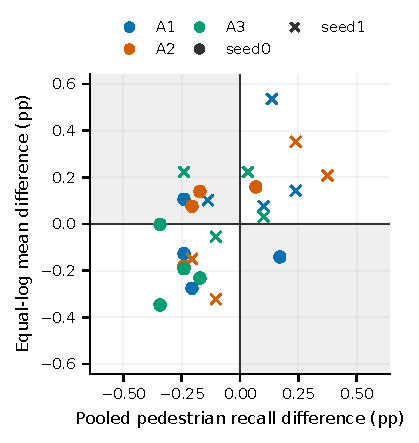
\includegraphics[width=\columnwidth]{images/gate_weighting.pdf}
\caption{All 24 complete candidate--control scopes: three arms, two seeds, and four conditions. Both axes are pedestrian-recall differences in percentage points. Shaded opposite-sign quadrants highlight weighting sensitivity. Each point uses the same 404 frames/eight logs, 198 pedestrian instances and 2,923 observations. Points are dependent descriptions, not independent experiments or confidence intervals.}\label{fig:weighting}
\end{figure}

\subsection{Why critical recall and AnyMiss disagree}
Table~\ref{tab:recovery} and Fig.~\ref{fig:recovery} add the complete saved-count decomposition. For A2/seed1/clean, 17 frames have fewer pedestrian misses and eleven have more. Their positive/negative count changes are 19/12, yielding seven additional hits. Every one of those 17 improved frames still misses at least one pedestrian. No joint frame becomes all clear and no previously all-clear joint frame fails: the 288 failed sample tokens are exactly the same. Joint VRU hits increase by only five because bicycle/motorcycle hits together decrease by two. Thus unchanged AnyMiss here is a lack of zero-miss boundary crossings, not a cancellation of changed failure identities.

The reverse disagreement also occurs. A2/seed1/LiDAR loses six pedestrian and three joint-VRU hits, yet AnyMiss improves from 292/307 to 291/307: one frame becomes all clear and none newly fails. A2/seed0/LiDAR loses six pedestrian hits, with 16 count-improved and 24 count-worsened frames, but no clear/new frame transitions. AnyMiss alone can therefore miss changes in failure severity in either direction. The original mAP/NDS/pedAP and output burdens remain as reported in Table~\ref{tab:agates}; they are not recomputed or averaged from folds.

Across all 24 complete A scopes, nine have positive pedestrian hit changes and fifteen negative changes. Six of the nine positive comparisons do not improve joint AnyMiss. Of fourteen unchanged-AnyMiss scopes, thirteen have zero clear/new transitions; one has one recovery offset by one new failure. These are dependent scope counts, not independent trials or a success-rate estimate. Across the same repeated comparisons, 268 frame-comparison occurrences have fewer pedestrian misses: 258 retain pedestrian misses, four retain only other-VRU misses, and six become jointly all clear. The occurrences are not 268 distinct independent frames.

Seed2's twelve valid-fold scopes are provided separately: pedestrian hits increase in four, decrease in five, and are unchanged in three; joint AnyMiss is unchanged in five. This is not full404 coverage or a three-seed mean. All four class/joint decompositions, 264 log comparisons, and 132 fold comparisons are supplied, with exact support and null SDK fields preserved.
\begin{table*}[t]
\centering\footnotesize
\caption{Exact saved-count decomposition of four diagnostic cases. C/L denote clean/LiDAR perturbation. A cases use 404 frames/eight logs, 198 pedestrian and 231 VRU instances; P2 is development-only (41 frames/one log/six pedestrian instances). G/D are sums of per-frame positive/negative pedestrian hit-count changes, not identified individual recovery/loss counts. Clear/New are exact joint-VRU frame transitions. Original detection metrics and output burden remain in Tables~\ref{tab:agates} and~\ref{tab:p}; the unavailable seed0/clean SDK effect remains null.}\label{tab:recovery}
\setlength{\tabcolsep}{4pt}
\begin{tabular}{lrrrrrrr}
\toprule
Case & Pedestrian hits $0\to1$/obs. & VRU hits $0\to1$/obs. & AnyMiss $0\to1$/target & Fewer/more frames & G/D & Clear/New & $\Delta$ped hits\\
\midrule
A2/s1/C & 1000$\to$1007/2923 & 1055$\to$1060/3333 & 288$\to$288/307 & 17/11 & 19/12 & 0/0 & +7\\
A2/s0/L & 983$\to$977/2923 & 1015$\to$1008/3333 & 292$\to$292/307 & 16/24 & 19/25 & 0/0 & -6\\
A2/s1/L & 960$\to$954/2923 & 996$\to$993/3333 & 292$\to$291/307 & 9/14 & 9/15 & 1/0 & -6\\
P2/dev & 8$\to$15/67 & 8$\to$15/67 & 30$\to$30/31 & 9/2 & 9/2 & 1/1 & +7\\
\bottomrule
\end{tabular}
\end{table*}

\begin{figure*}[t]
\centering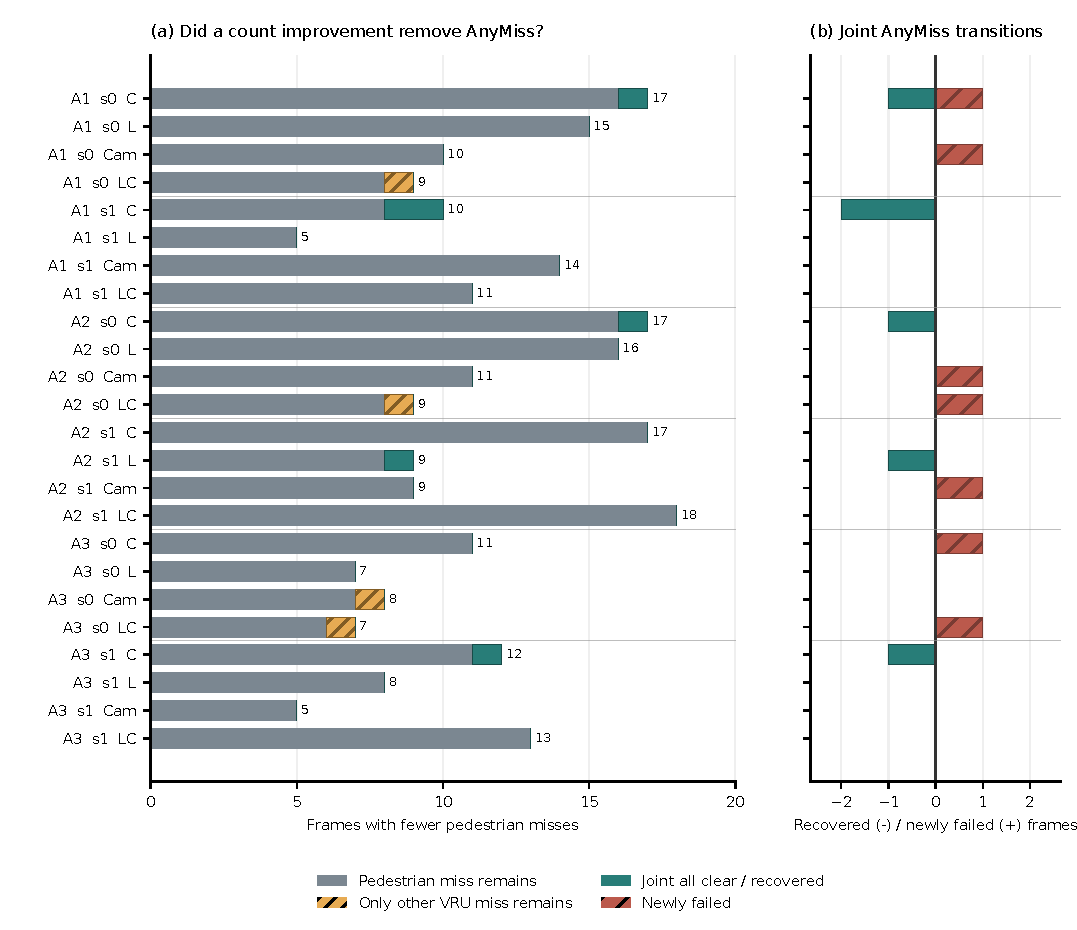
\includegraphics[width=\textwidth]{images/recovery_frame_transitions.pdf}
\caption{All 24 complete A1--A3/A0 scopes, each using the same 404 frames/eight logs, 2,923 pedestrian observations/198 instances, and 3,333 joint-VRU observations/231 instances. C/L/Cam/LC denote clean, LiDAR, camera, and combined conditions. Left: frames with fewer pedestrian misses, classified by residual failures. Right: exact joint all-clear recoveries (negative) and newly failed frames (positive); these are counts, not signed probabilities. Bars do not identify individual target turnover. Seed2's incomplete cohort is kept in the accompanying valid-fold tables.}\label{fig:recovery}
\end{figure*}

\subsection{A local detection-metric disagreement}
The original fixed-8,000-update P2 clean development screen changes mAP from 2.1758\% to 2.5328\% and NDS from 7.2406\% to 9.2326\%. Pedestrian AP remains zero, critical pedestrian/joint hits increase from 8/67 to 15/67, and AnyMiss remains 30/31 target frames. One recovered and one newly failed frame leave the total unchanged. Table~\ref{tab:p} preserves output burden and the small one-log/six-instance support. The aggregate AP gain comes from car/cone with a truck decrease, not improved pedestrian AP. It is a historically exposed development observation and cannot rescue promotion after mandatory P1 execution failure.

R2 locates the count changes: nine frames have fewer misses and two have more, giving positive/negative changes of 9/2. Eight improved frames still fail. A single-target frame recovers while another single-target frame newly fails; 29 frames remain failed (eight with fewer, one with more, twenty with equal miss counts). This differs from A2/seed1/clean, whose failed-frame identities never change. P2's actual target-observation recovery/loss counts are bounded by $R\in[9,15]$, $L\in[2,8]$, coupled by $R-L=7$. A2/seed1/clean has wider bounds $R\in[19,845]$, $L\in[12,838]$, also with $R-L=7$. Calling the lower bounds exact recovered/lost people would overstate what the archive retains.
\begin{table*}[t]
\centering\footnotesize
\caption{Matched fixed-8,000-update clean development screen only.}\label{tab:p}
\setlength{\tabcolsep}{3pt}
\begin{tabular}{lrrrrrrrrr}\toprule
Detector & mAP\% & NDS\% & PedAP\% & Ped hits & VRU hits & AnyMiss target & All frames & Ped out. & Ped unm.\\\midrule
B1 fixed 8k & 2.1758 & 7.2406 & 0.0000 & 8/67 & 8/67 & 30/31 & 30/41 & 2175 & 2165\\
P2 fixed 8k & 2.5328 & 9.2326 & 0.0000 & 15/67 & 15/67 & 30/31 & 30/41 & 2177 & 2160\\
\bottomrule\end{tabular}
\par\vspace{3pt}\begin{minipage}{0.98\textwidth}\footnotesize Each row: F0/seed0, 41 frames, 1 log, 6 critical pedestrian instances, 67 observations; 31 target frames. Motorcycle/bicycle support 0, three-class macro unresolved. Both states uncalibrated. Outputs/unmatched at score$\geq0.1$ are all-range diagnostics, not official FP/precision. One recovered and one new AnyMiss frame leave the count unchanged; no outer promotion.\end{minipage}
\end{table*}


\subsection{Risk scores do not improve consistently}
Table~\ref{tab:risk} gives every seed under full-frame, target-frame, and equal-log scoring. Relative to the development-prevalence baseline, full404 Brier/NLL changes are $+0.097650/+0.388724$, $+0.021748/+0.064392$, and $-0.009245/-0.010828$ for seeds 0--2. Two seeds worsen. Seed2's small pooled advantage reverses under equal-log weighting: Brier changes from 0.267446 to 0.268341 and NLL from 0.922289 to 0.931540. All three equal-log comparisons worsen on both losses (Fig.~\ref{fig:risk}). The target-only stratum also lacks a consistent gain.

For all404, the fixed $q=0.5$ reference has Brier 0.25 and NLL 0.693147. All three candidate NLLs are worse than this reference. Seed2's Brier is only slightly below 0.25 and does not imply robust monitoring. R1 alone evaluates no alarm policy or ranking endpoint; the R3 extension below addresses these separately. No coverage guarantee or collision-risk interpretation follows. The original B2/B3 risk fields remain null; R1--R3 are separately labelled internal analyses. There is no new detector update, GPU execution, SDK evaluation, or change to mAP/recall/AnyMiss.
\begin{table*}[t]
\centering\footnotesize
\caption{Fixed monitor scores; lower Brier/NLL is better. All seeds and declared scopes are shown.}\label{tab:risk}
\setlength{\tabcolsep}{3pt}
\begin{tabular}{llrrrrrr}\toprule
Scope & Seed & Const. Brier & Monitor Brier & $\Delta$Brier & Const. NLL & Monitor NLL & $\Delta$NLL\\\midrule
Full404 & 0 & 0.275350 & 0.373000 & +0.097650 & 0.884444 & 1.273168 & +0.388724\\
Full404 & 1 & 0.258868 & 0.280616 & +0.021748 & 0.855498 & 0.919890 & +0.064392\\
Full404 & 2 & 0.259172 & 0.249927 & -0.009245 & 0.867522 & 0.856694 & -0.010828\\
Target307 & 0 & 0.171024 & 0.273844 & +0.102820 & 0.535739 & 0.909421 & +0.373682\\
Target307 & 1 & 0.143362 & 0.194701 & +0.051339 & 0.484779 & 0.603868 & +0.119089\\
Target307 & 2 & 0.131977 & 0.129628 & -0.002348 & 0.468314 & 0.435056 & -0.033258\\
Equal-log & 0 & 0.289153 & 0.409802 & +0.120649 & 0.947197 & 1.402110 & +0.454913\\
Equal-log & 1 & 0.266280 & 0.309417 & +0.043137 & 0.906077 & 1.020997 & +0.114920\\
Equal-log & 2 & 0.267446 & 0.268341 & +0.000895 & 0.922289 & 0.931540 & +0.009251\\
\bottomrule\end{tabular}
\par\vspace{3pt}\begin{minipage}{0.98\textwidth}\footnotesize Each seed uses the same eight outer logs: 404 frames, with 270/272/266 AnyMiss events for seeds 0/1/2. Target307 uses only the original target-containing stratum with the same event numerators. Equal-log first computes each log loss, then averages eight logs equally. Const. is the corresponding development prevalence. The monitor includes nine actual fits and three predetermined constant fallbacks. NLL uses natural logs; no iid intervals, seed-averaged inference, new detection, SDK, or acceptance policy is implied.\end{minipage}
\end{table*}

\begin{figure}[t]
\centering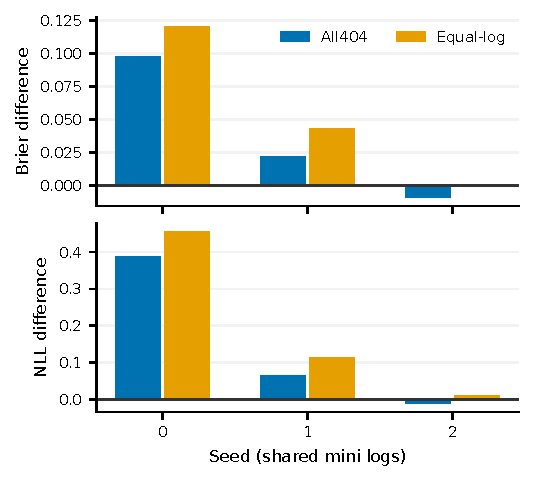
\includegraphics[width=\columnwidth]{images/risk_differences.pdf}
\caption{Fixed monitor minus development-prevalence baseline. Positive loss differences are worse. Blue uses all404 frames; orange gives each of eight logs equal weight. No error bars or inferential intervals are claimed. Seed2's small pooled advantage does not survive equal-log weighting.}\label{fig:risk}
\end{figure}

\subsection{Ranking does not yield consistent budgeted screening}
Table~\ref{tab:ranking} retains all scores and seeds. Each seed uses the same 404 frames/eight logs, with 270, 272, and 266 original AnyMiss failures. LR captures 57.58/270, 43.56/272, and 51.47/266 expected failures at 80/404 alarms, against same-volume random expectations of 53.47, 53.86, and 52.67. LR exceeds Dev in all three seeds and Conf in two, but random in only seed0. A comparison limited to the weak pooled Dev baseline would overstate screening utility. The frozen consistency criterion fails.

The whole curve gives a different description (Fig.~\ref{fig:r3coverage}). LR AUROC is 0.4596/0.5353/0.5704; LR AURC is 0.7282/0.6131/0.5695, compared with Dev's 0.7126/0.6762/0.6260. Thus seed1/2 show some curve-level signal, whereas seed0 worsens. This cannot replace a specified operating budget. Equal-log primary capture-minus-alarm fractions are $-2.78/+2.28/-0.85$ percentage points for LR; only six of eight logs per seed support AUROC. Within-log constants remain nondiscriminating even when pooled fold prevalence differs.

The target307 diagnostic does not establish an alternative success: at 61 alarms LR captures 51.87/53.00/53.62 expected failures, random expects 53.65/54.05/52.85, and Conf captures 56/57/57. High target-stratum $\mathrm{AP}_{risk}$ accompanies high failure prevalence and is not evidence of safe acceptance. Full precision, all diagnostic budgets, and every log/fold are provided digitally.
\begin{table}[t]
\caption{Frozen-score ranking and primary alarm budget. Each seed has 404 frames/eight logs; all rows flag exactly 80 expected frames (19.802\%). LR is the saved logistic/fallback score; Dev is development prevalence; Conf is one minus maximum pedestrian confidence. $\mathrm{AP}_{risk}$ is threshold-grouped failure AP, distinct from detector mAP/pedAP. Lower AURC is better. Capture counts are uniform boundary-tie expectations; random uses the same 80 alarms, not an AP reference.}
\label{tab:ranking}
\centering\footnotesize
\setlength{\tabcolsep}{2.6pt}
\begin{tabular}{ccrrrrr}\toprule
Seed & Score & AUROC & $\mathrm{AP}_{risk}$ & AURC & Capture/$P$ & Random\\\midrule
0 & LR & 0.4596 & 0.6910 & 0.7282 & 57.58/270 & 53.47 \\
0 & Dev & 0.4390 & 0.6413 & 0.7126 & 40.49/270 & 53.47 \\
0 & Conf & 0.4136 & 0.6159 & 0.7463 & 47.00/270 & 53.47 \\
1 & LR & 0.5353 & 0.6720 & 0.6131 & 43.56/272 & 53.86 \\
1 & Dev & 0.4568 & 0.6423 & 0.6762 & 39.51/272 & 53.86 \\
1 & Conf & 0.3702 & 0.6062 & 0.7784 & 46.00/272 & 53.86 \\
2 & LR & 0.5704 & 0.7004 & 0.5695 & 51.47/266 & 52.67 \\
2 & Dev & 0.4907 & 0.6414 & 0.6260 & 36.54/266 & 52.67 \\
2 & Conf & 0.3898 & 0.5755 & 0.7323 & 35.00/266 & 52.67 \\
\bottomrule\end{tabular}
\end{table}

\begin{figure*}[t]
\centering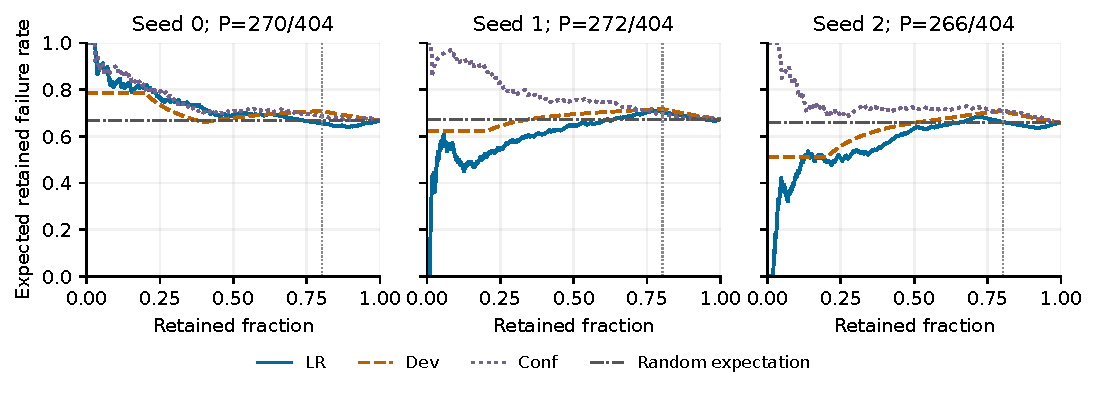
\includegraphics[width=\textwidth]{images/risk_ranking_coverage_r3.pdf}
\caption{R3 descriptive risk--coverage curves using all 3,636 saved points and uniform expected tie allocation. Coverage retains the lowest-risk frames; the outcome is any critical-VRU miss, not collision risk. Horizontal lines show each seed's analytic random-retention failure rate. The vertical line is 324/404 retained (80 alarms). All seeds use the same eight logs with dependent observations; pooled scores mix fold models. No smoothing, iid confidence bands, calibrated-risk bound, or executed rejection policy is claimed. Lower curves at one coverage do not imply improvement at every alarm budget.}\label{fig:r3coverage}
\end{figure*}

\subsection{Development-fixed alarms show limited enrichment and burden drift}
Table~\ref{tab:fixedpolicy} gives all nine fixed-policy descriptions. LR's outer alarm fractions become 40.97\%, 23.90\%, and 39.49\%, although development cutoffs target about 20\%. Expected captures are 115.36/270, 78.18/272, and 113.64/266; excess above random at each actual alarm volume is $+4.73/+13.18/+8.60$. These are limited internal enrichment signals, not gains at a fixed 20\% outer budget. Ratios of expected unflagged failures to expected unflagged frames are 64.85\%, 63.04\%, and 62.32\%; an unflagged frame cannot be interpreted as safe.

An explicitly diagnostic decomposition of these saved operating points shows concentration. Summing within-log excess captures at each log's same alarm volume gives $+11.61/+12.59/+10.73$, but positive/negative/zero-enrichment logs number 1/3/4, 2/1/5, and 3/1/4. Equal-log mean capture-minus-alarm fractions are $+0.60/+1.73/-0.04$ points. Aggregation therefore still matters, and seed2 lacks an equal-log advantage. These diagnostics are not substituted for the failed primary criterion. There is no subsequent candidate expansion, refit, or selected winning budget.
\begin{table*}[t]
\caption{Development-fixed alarm policy on all404 outer frames, eight logs per seed. Each fold's cutoff and tie probability use only development scores, aiming at $\lfloor0.2n_{dev}\rfloor$ alarms. Outer alarm volume is observed rather than forced to 20\%. $P$ is the original AnyMiss failure count (270/272/266). Every numerator with a decimal is an expected count under label-independent tie allocation, not a fractional physical frame. Last column is excess captured failures above analytic random alarms at that row's same outer alarm volume. Rates are ratios of expected counts, not expectations of ratios under a random policy. All baselines/seeds are retained. These retrospective descriptions have no deployment or calibration guarantees.}
\label{tab:fixedpolicy}
\centering\small
\setlength{\tabcolsep}{5pt}
\begin{tabular}{ccrrrrr}\toprule
Seed & Score & Expected alarms/$N$ & Alarm \% & Expected capture/$P$ & Unflagged failures/frames & Excess vs. random\\\midrule
0 & LR & 165.54/404 & 40.97 & 115.36/270 & 154.64/238.46 & +4.73 \\
0 & Dev & 77.56/404 & 19.20 & 52.04/270 & 217.96/326.44 & +0.21 \\
0 & Conf & 125.00/404 & 30.94 & 71.00/270 & 199.00/279.00 & -12.54 \\
1 & LR & 96.54/404 & 23.90 & 78.18/272 & 193.82/307.46 & +13.18 \\
1 & Dev & 77.56/404 & 19.20 & 52.45/272 & 219.55/326.44 & +0.23 \\
1 & Conf & 126.00/404 & 31.19 & 66.00/272 & 206.00/278.00 & -18.83 \\
2 & LR & 159.54/404 & 39.49 & 113.64/266 & 152.36/244.46 & +8.60 \\
2 & Dev & 77.56/404 & 19.20 & 51.32/266 & 214.68/326.44 & +0.26 \\
2 & Conf & 115.00/404 & 28.47 & 60.00/266 & 206.00/289.00 & -15.72 \\
\bottomrule\end{tabular}
\end{table*}


\section{Completion, provenance, and reproducibility}
The distinction between completed negative findings and unperformed experiments is material (Table~\ref{tab:status}). The original A matrix has sixteen missing F0/seed2 groups after a damaged trajectory. Its known update lower bound is 209,607; the exact global count and unknown-suffix cardinality remain null. The 227,400 reservation within 228,000 is not actual cost or a spare training budget. The unavailable seed0/A0/clean SDK result and its dependent effects stay null. Complete A full404 analysis uses only two seeds; seed2's 48 valid-fold groups cover 243 frames and six logs and are not a full404 or three-seed mean.

B1 training and its 96 original LOLO evaluations are complete. Twelve full404 results are exact historical reuse, not new evaluations. In its LiDAR-only implementation, camera/clean and combined/LiDAR pairs have equal metrics and counts in all original full/omission scopes; no implemented camera-fusion benefit follows.

P1 is a warranted execution failure with 1,063 known updates, 1,000 saved, and actual count in $[1063,1064]$; it is not an algorithmic negative result. Its recorded sequence is JSON-reading failure, TERM/KILL, and child exit $-9$, without an established underlying cause. Permanent original \code{NO_PROMOTION} prevents eleven additional winner screens and promoted outer inference. B2/B3 remain conditionally stopped following an actual 256 MiB consumer boundary, missing required class support in nine of twelve development groups, and incomplete physical camera projection/fusion wiring. Unpublished in-memory comparisons are not results. None of these experiments is currently running or silently resumed for this revision.
\begin{table}[t]
\centering\footnotesize
\caption{Terminal outcomes versus unperformed work.}\label{tab:status}
\begin{tabular}{>{\raggedright\arraybackslash}p{0.27\columnwidth}>{\raggedright\arraybackslash}p{0.63\columnwidth}}\toprule
Component & Actual disposition\\\midrule
Original A & Terminal with damaged F0/seed2; 176/192 primary groups. No replay.\\
B1 / LOLO & Training and original 96 LOLO evaluations complete.\\
P1 / promotion & Warranted execution failure; original NO\_PROMOTION permanent. Winner/outer extensions unperformed.\\
B2/B3 & Conditional stop: resource boundary, absent support and incomplete fusion implementation.\\
R1 log/risk & Complete: 192 paired-log descriptions; nine fits plus three fallbacks; no stable gain.\\
Independent replication & Not yet performed by an external person/team. Compact reproduction is available.\\
New GPU search & Not started; stopped this round under the fixed stopping rule.\\\bottomrule
\end{tabular}
\end{table}


The R1 pilot reads 48 exact saved prediction/endpoint files, totaling 456,293,997 bytes; its controlled phase reads including declared preparation carry total 484,431,389 bytes, below a 1 GiB phase cap. This is not total-task or physical I/O. The pilot script reports about 3.172 s wall and 2.906 s process CPU, excluding other research/report operations. A missing-pin preparation failure and its consumed bytes are preserved. A Windows memory-API wrapper returned an unusable zero: actual RSS is null and the intended 2 GiB observed-RSS guard was not verified. The original END is retained with an explicit erratum, without a scientific rerun to repair it.

Saved-model inference reconstructs all 1,212 outer probabilities with maximum absolute discrepancy $1.67\times10^{-16}$. Separate scalar checks of normalization, role assignments, objective gradients, Brier/NLL, and paired counts are retained. They are same-author numerical checks, not external independent replication. Figure/table creation reads these accepted compact values; it performs no refit, GT matching, input recapture, SDK replay, or raw-backup replay.

R2's original saved counts reconcile with all 176 selected fold descriptions and all 256 available full404 selected per-log rows. A separately written scalar verifier checks 3,996 decomposition quantities and exhaustively enumerates possible hit-set identities for 140 count configurations with $n\le6$ to verify the count-only bounds. These checks do not recreate absent match identities or provide external replication. An initial parser failed on the preserved SDK \code{null} string; its source, compact-read cost, and failure are retained. A successor fixes only null parsing, with no reread of the 179 endpoint/cohort sources and no SDK retry. Preliminary console-encoding failure and non-exact preledger metadata cost are also retained. Exact bounded source-return accounting is separated from total-task or physical I/O.

R3 reads seventeen exact compact R1 sources totaling 2,309,190 bytes, with source hashes and before/after state checks. Saved outer probabilities are retained unmodified. A separately written same-author verifier checks 27,741 quantities using pairwise AUROC, direct threshold AP, exact rational tie prefixes, all operating points, and 64 finite label/score configurations covering 496 tie permutations. This is not external independent replication, statistical confirmation, or a rerun of the original evaluator. Controlled returned-byte costs are separated from physical and total-task I/O.

The reproduction package contains original R1 compact inputs, models and probabilities; R2's paired counts and all available scope/class decompositions; and R3's frozen protocol, 36 development rules, every log/fold/budget, all curve points, source hashes and numerical checks. Read-only standard-library verification entry points operate on compact copies. Preserved prior report packets supply detector settings, evidence, and authoring versions. Large prediction files and checkpoints remain in the original archive. An optional exact CPU monitor refit in the prior R1 packet is clearly separated and was not rerun. Compilation and document value checks do not constitute new scientific validation.

\section{Limitations and prioritized further work}
\subsection{What the findings establish}
This case demonstrates that the scientific description can change with aggregation weights and with observation-count versus frame-event endpoints, that class coverage does not ensure both binary-event labels are present, and that a fixed monitor can fail despite numerically correct fitting. The saved-count decomposition distinguishes residual failures from cancellation of newly failed/recovered frames. R3 additionally distinguishes probability losses, overall ranking, fixed-budget screening, and the burden of development-fixed alarms. Some internal enrichment exists, but it does not overturn the failed consistency criterion. These are applications of established evaluation principles to an inspected BEV pipeline. A sign reversal or elementary count identity is not an algorithmic discovery; a traceable archive alone is not proof of scientific novelty. The empirical contribution depends on the transparent, complete case analysis.

The mini dataset has eight logs, repeated frames/instances, overlapping fold training, and historical/adaptive exposure. Three risk seeds are trained replicas on the same logs, not three independent datasets. We give no default iid-frame bootstrap, $p$-value, or population confidence interval. Log omission and equal-log means remain descriptive. Additional seeds or another split of the same exposed mini cannot create fresh external validation.

Detection baselines have low absolute AP. A controls differ in parameterization and have a decoder LiDAR path; B1 is a different architecture with no connected camera path. Missing A groups, one missing SDK baseline, and P1 execution failure restrict estimable effects. The simple clean-only monitor uses pedestrian features to predict joint VRU failure; it does not test richer geometry, class-specific monitors, perturbation robustness, calibration guarantees, or general risk-model impossibility. Its one-log development fitting is especially fragile. R3's illustrative 20\% budget is not a driving requirement. Mixed-fold ranking, expected tie allocation, and observed development-threshold transfer are retrospective diagnostics. A qualified selective policy still needs independently supported coverage/risk evaluation \cite{Geifman2017Selective}; no deployment guarantee or safety claim is supplied.

\subsection{Directions with realistic expected value}
An independent person should reproduce compact inputs-to-scores and the saved-count decomposition, and verify roles without accessing original evaluators. A same-author clean-environment repeat alone must not be renamed independent replication. R2 completes the available frame-level recovery/new-failure analysis, but per-instance match status was not retained. Exact individual turnover, consecutive-person miss trajectories, and within-frame identity exchanges remain unidentifiable without an additional matching operation, which is outside this study. Future evaluations should persist immutable matched annotation/instance identities at the original endpoint computation, rather than reconstruct them from aggregate counts.

A stronger detector with matched controls, genuinely independent new capture logs, and sufficient positive/negative monitor events would test transferability. For monitoring, freeze the score and alarm policy before new logs, then report actual alarm burden, failure capture, residual failures, and log-level heterogeneity together. These require a new bounded design and data, not unbounded candidate search on the same mini. R3 completes the authorized existing-score analysis and ends candidate expansion. Completing physical projection/fusion, repeating the finer-grid screen, filling the damaged matrix, or restarting B2/B3 is outside this revision and cannot be inferred from GPU availability. No stable improvement is promised for these directions, and the original consumed budgets are not reopened.

\section{Conclusion}
The revised study supports a limited evaluation contribution: paired log descriptions expose aggregation sensitivity; saved frame counts explain recall/AnyMiss disagreement through residual misses and offsetting frame transitions; and a role-preserving monitor lacks consistent probability-score or fixed-budget screening improvement. Development-fixed alarms show limited internal enrichment with substantial burden drift and log concentration. Frame transitions are identified, while unsaved individual match identities impose target-turnover bounds. Detection quality, critical recall, frame failures, probability loss, ranking, and alarm burden remain distinct. Original failures and missingness are preserved; R1--R3 do not overturn \code{NO_PROMOTION}. Stable gate efficacy, deployable risk monitoring, and external generalization remain unresolved.

\balance
\bibliographystyle{IEEEtran}
\bibliography{references}
\end{document}

